% !TeX root=../main.tex
\chapter{مروری بر مطالعات انجام شده}
%\thispagestyle{empty} 
\section{مقدمه}
در این فصل به مرور تعدادی از مقالات مربوط به استراتژی ذخیره‌سازی و سیاست جایگزینی محتوا در حافظه برای شبکه‌های اینترنت اشیا می‌پردازیم. در ادامه الگوریتم‌های استفاده شده در مقالات، معماری به کار رفته برای پیاده‌سازی و چالش‌های آن برای محیط  استفاده شده به طور اجمالی بیان می شوند. 

\section{مروری بر ادبیات موضوع}

\subsubsection{\lr{Caching Transient Content for IoT Sensing: Multi-Agent Soft Actor-Critic}}
در مقاله‌ی \cite{wu2021caching} برای اولین بار راه حلی برای مسئله‌ی به روز رسانی حافظه‌ی کش برای یک محیط چندعامله و متشکل از چندین گره لبه ارائه شده و این مسئله به صورت یک فرآیند تصمیم‌گیری مارکوف مشارکتی بین چندعامل براساس کاهش مقدار تابع وزنداری از طول عمر آیتم هر محتوا، هزینه‌ی به روزرسانی حافظه‌ی ذخیره‌سازی، بارترافیکی شبکه و کاهش مصرف انرژی در واکشی پاسخ مطرح گردیده است. 

در اینجا یک نسخه از الگوریتم چندعامله‌ی \lr{Soft Actor-Critic} با فضای اعمال گسسته ایجاد شده است که تعداد عامل‌های الگوریتم خروجی به طور خطی با تعداد گره‌های لبه و حسگرهای شبکه‌های اینترنت اشیا قابل افزایش است. برای رسیدن به این هدف، در این مقاله از یک \lr{Gumble-SoftMax-sampler} برای نمونه‌برداری از محیط استفاده شده است که پارامترهای مربوط به آن را برای رسیدن به فضای اعمال دیفرانسیل‌پذیر تنظیم می‌نماید. در آخر نیز برای برقرای توازن میان اکتشاف و بهره‌وری (که مسئله‌ی مشترک میان تمامی الگوریتم‌های یادگیری تقویتی می‌باشد) از یک تنظیم‌ساز آنتروپی\footnote{\lr{Entropy Regularization}} برای جلوگیری از همگرایی زودهنگام استفاده می‌شود.

برای کاهش سربار ارتباط میان گره‌های لبه و لایه‌ی ابری، هریک از الگوریتم‌های \lr{Soft Actor-Critic} و \lr{Deep Q-Network} در دو حالت روش کنترلی متمرکز و غیرمتمرکز پیاده‌سازی و مقایسه شده‌اند. در سیاست کنترلی غیرمتمرکز\ref{fig:decentralized}، هرکدام از سرورهای گره‌های لبه به عنوان یک عامل مستقل، براساس مشاهدات خود تصمیماتی را برای ذخیره‌کردن، جایگزینی محتوا و ... اتخاذ می‌نماید اما در روش کنترلی متمرکز\ref{fig:centralized} از یک پردازنده‌ی ابری\footnote{\lr{Cloud Processor}} برای بهبود پاداش‌های دریافتی سیستم و بالا بردن هماهنگی با سایر گره‌های لبه استفاده می‌شود.

\begin{figure}[ht]
	\centering 
	\subfloat[روش کنترلی متمرکز]{ \label{fig:centralized}
		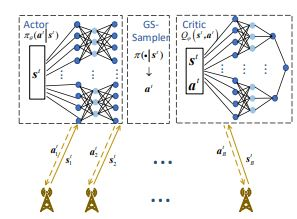
\includegraphics[width=0.4\textwidth]{centralized}}
	\hspace{2mm}
	\subfloat[روش کنترلی غیرمتمرکز]{ \label{fig:decentralized}
		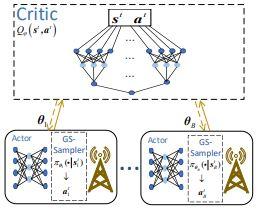
\includegraphics[width=0.4\textwidth]{decntralized}}%
	\caption{دیاگرام الگوریتم \lr{SAC} به کاررفته}
	\label{fig:centralizedvsdec} %% label for entire figure
\end{figure}

همانطوری که در شکل \ref{fig:centralizedvsdec} دیده می‌شود، در الگوریتم متمرکز، پردازنده‌ی ابری نقش یک عامل متمرکز را ایفا می‌کند و سیاست متمرکز برای تمامی گره‌های لبه را یاد می‌گیرد. متناسباً هریک از گره‌های لبه ابتدا مشاهدات خود را در هر واحد زمانی برای پردازنده‌ی ابری می‌فرستند و سپس پس از آنکه پردازنده‌ی ابری مشاهدات محلی آنها را جمع‌آوری کرد، عملکرد بهینه برای هریک از گره‌های لبه را ارسال می‌نماید. 

در آخر نیز، عملکرد الگوریتم \lr{SAC} در حالت متمرکز و غیر متمرکز با روش‌های عملگر-نقاد معمول و روش \lr{DQN} مقایسه شده است. به طور کلی، متوسط پاداش دریافتی برای \lr{Decentralized SAC} نسبت به \lr{Centralized SAC} بیشتر بوده و مقدار به دست آمد حاصل از الگوریتم \lr{Centralized SAC} از الگوریتم عملگر-نقاد معمول بیشتر بوده و برای الگوریتم عملگر-نقاد معمول نسبت به \lr{DQN} بیشتر است و البته باید به این نکته اشاره کرد که متوسط پاداش به دست آمده برای الگوریتم \lr{DQN} نسبت به سایر الگوریتمها نویزی تر نیز می‌باشد. 


%\begin{figure}[ht]
%	\centerline{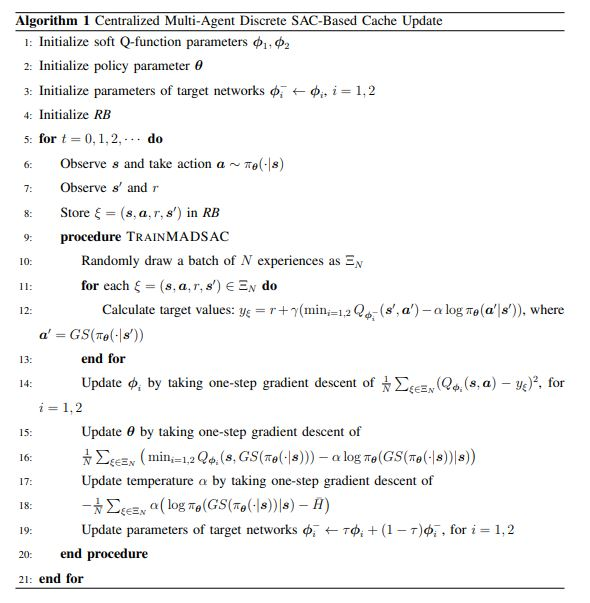
\includegraphics[width=8cm]{centralizedSAC}}
%	\caption{الگوریتم \lr{Centralized Soft Actor-Critic}}
%	\label{fig:cSACAlgo}
%\end{figure}

%\begin{figure}[ht]
%	\centerline{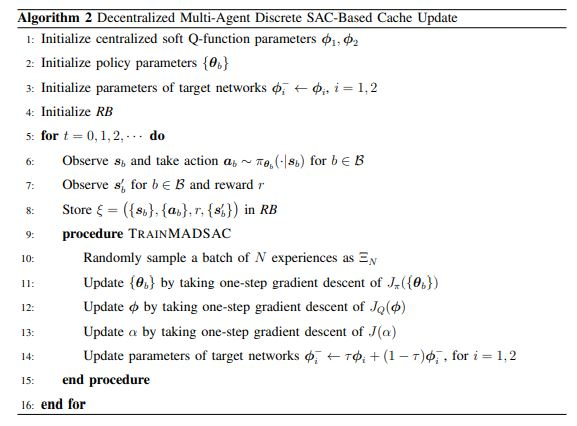
\includegraphics[width=8cm]{decentralizedSAC}}
%	\caption{الگوریتم \lr{Decentralized Soft Actor-Critic}}
%	\label{fig:dSACAlgo}
%\end{figure}

\subsubsection{\lr{Deep Reinforcement Learning for Cooperative Content Caching in Vehicular Edge Computing and Networks}}
با توجه به ماهیت محیط و حرکت گره‌های مصرف کننده،‌در مقاله‌ی \cite{qiao2019deep} تعریف حالت با آنچه که پیشتر دیدم تفاوت‌هایی دارد، در ضمن فضای اعمال مجاز نیز دیگر گسسته نخواهد بود که بتبع این مسئله پیچیدگی‌های بسیاری را به وجود می آورد. در ابتدا درباره‌ی فضای حالات و اعمال توضیحاتی داده می‌شود:

\paragraph{فضای حالات}
در ابتدای هر بازه‌ی زمانی، عامل هوشمند به اطلاعاتی در باره‌ی محتوای درخواستی توسط وسایل نقلیه\footnote{\lr{content requesting vehicles(CRV)}} دست پیدا می‌کند که این اطلاعات حالت عامل در این بازه‌ی زمانی را برای ما مشخص می‌کند و این مولفه‌ها عبارتند از:  
\begin{itemize}
	\item 
	نوع محتوای درخواست شده در بازه‌ی زمانی ذخیره‌سازی 
	\item 
	مهلت تحویل دیتای درخواستی در بازه‌ی زمانی ذخیره‌سازی کنونی
	\item
	سایز باقیمانده از دیتای درخواستی برای ارسال در بازه‌ی زمانی کنونی
	\item
	مولفه‌ی مربوط به منطقه‌ای که دیتای مربوط به محتوای درخواستی موجود بوده یا مولفه‌ی مربوط به موقعیتی که دیتای درخواستی ذخیره شده است.
	\item 
	میزان محبوبیت محتوای درخواستی در بازه‌ی زمانی فعلی
	\item 
	بیانگر عملیات ذخیره‌سازی\footnote{\lr{caching indicator}} که نشان می‌دهد در بازه‌ی زمانی ذخیره‌سازی فعلی، دخیره‌ی دیتای درخواستی در کدام گره ذخیره‌سازی انجام شود.
\end{itemize}

\paragraph{فضای اکشن‌ها}
بعد از دریافت درخواست محتوا، رسانه‌ی همه‌پخشی ماهواره‌ای\footnote{\lr{Media Broadcast Satellite(MBS)}} محبوبیت محتوای درخواست شده را محاسبه می‌کند و از روی آن تصمیم می‌گیرد که‌آیا لازم است دیتای مربوط به محتوای درخواستی ذخبره شود یا خیر و در صورتیکه پاسخ مثبت باشد،‌ گره مناسب برای ذخیره‌ی دیتا را مشخص می‌نماید. در هر بازه‌ی زمانی مربوط به واکشی پاسخ، مقادیر زمان‌بندی برای هریک از وسایل و نیز پهنای باند تخصیص یافته به هرکدام، توأماً برای کاهش هزینه‌ی دسترسی به محتوا با قید مهلت مربوط به ارسال پاسخ مورد استفاده قرار می‌گیرند. بنابراین فضای اکشن‌ها با مولفه‌هایی که در ادامه توصیف می‌شوند، مشخص می‌گردد.
\begin{itemize}
	\item 
	آیا محتوای درخواستی در بازه‌ی زمانی ذخیره‌سازی در حافظه وجود داشته است یا خیر. در صورتیکه جواب مثبت باشد، مقدار این مؤلف 1 خواهد بود.  
	\item 
	نشانگر ارتباط\footnote{\lr{association indicator}} بین محتوای درخواستی و گره لبه، در واقع این مولفه مشخص می‌کند تا برایواکشی پاسخ باید به سراغ کدامیک از گره‌های لبه برویم.
	\item
	پهنای باندی که به ازای آن ارتباط بین گره لبه و وسیله‌ی درخواست دهنده برقرار می‌شود.
\end{itemize}
 
 در اینجا با توجه به پیوسته بودن فضای استیت‌ها و به طور ویژه اکشن‌ها به جای تخمین ارزش استیت ها یا ارزش استیت‌-اکشن‌ها (که به کمک شبکه یا شبکه‌ها‌ی عصبی صورت می‌پذیرد) ، به طور مستقیم سیاست بهینه را با استفاده از الگوریتم \lr{Deep Deterministic Policy Gradient}(\ref{fig:DDPG}) تخمین می‌زنیم.
 \begin{figure}[ht]
 	\centerline{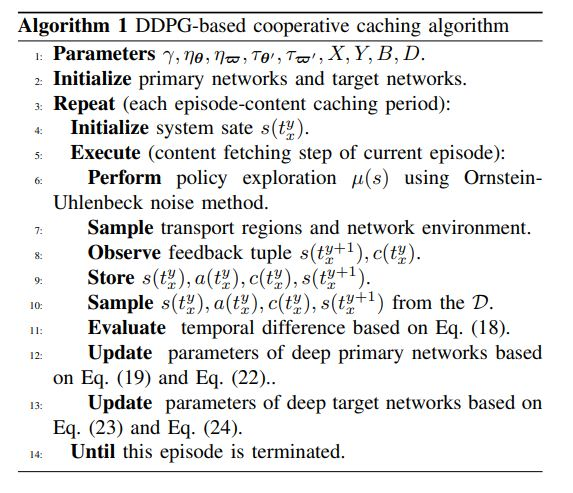
\includegraphics[width=11cm]{DDPG}}
 	\caption{الگوریتم \lr{Deep Deterministic Policy Gradient}}
 	\label{fig:DDPG}
 \end{figure}

الگوریتم پیشنهادی مقاله در زمره‌ی یادگیری بدون مدل به‌ شمار می‌رود که براساس تعداد بسیاری از تجربیات و تعاملات با محیط، تخمین سیاست صورت می‌پذیرد.  
\begin{figure}[ht]
	\centerline{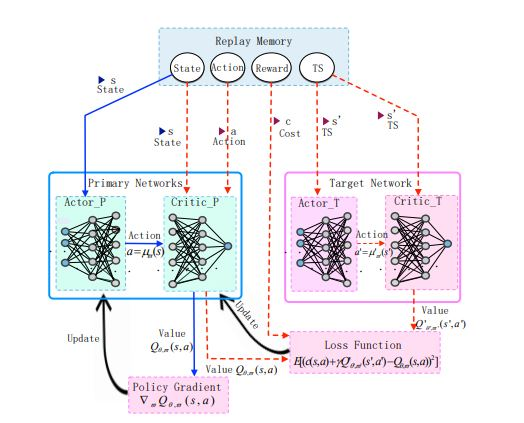
\includegraphics[width=10cm]{PG}}
	\caption{دیاگرام \lr{Deep Deterministic Policy Gradient}}
	\label{fig:PG}
\end{figure}



\subsubsection{\lr{A Deep Reinforcement Learning-Based Caching Strategy for IoT Networks with Transient Data}}


\begin{figure}[ht]
	\centerline{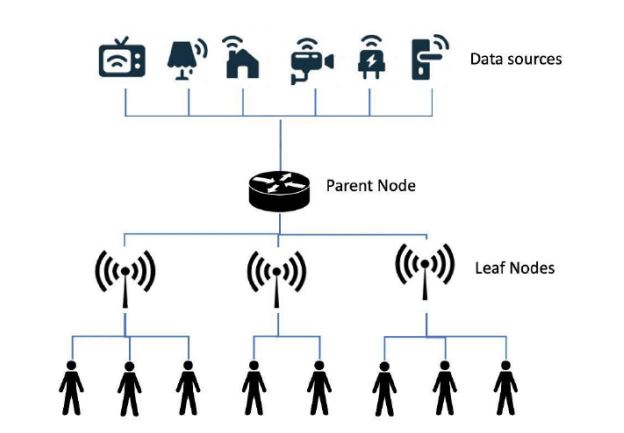
\includegraphics[width=10cm]{parent-leaf}}
	\caption{نمایی از معماری ریشه-برگ}
	\label{fig:parent-leaf}
\end{figure}

\begin{figure}[ht]
	\centerline{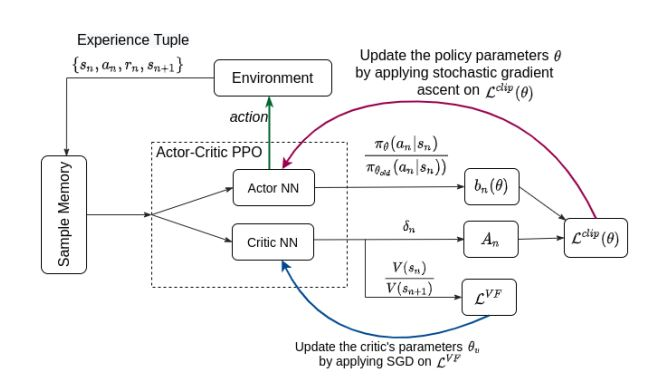
\includegraphics[width=10cm]{PPO-diagram}}
	\caption{دیاگرام \lr{Proximal Policy Optimization}}
	\label{fig:ppod}
\end{figure}

\begin{figure}[ht]
	\centerline{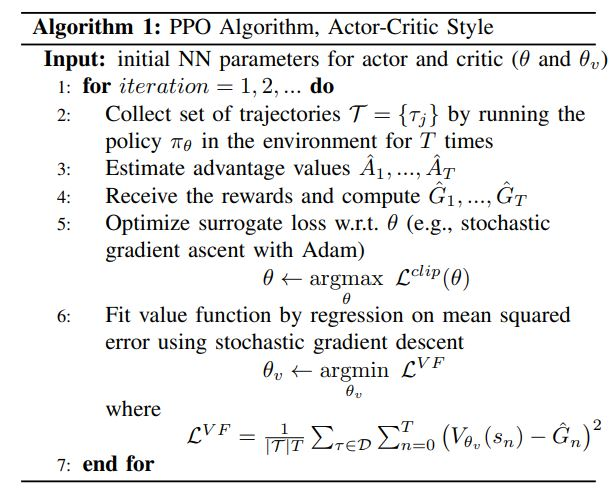
\includegraphics[width=10cm]{PPO}}
	\caption{الگوریتم \lr{Proximal Policy Optimization}}
	\label{fig:ppo}
\end{figure}

\subsubsection{\lr{HFDRL: An Intelligent Dynamic Cooperate Cashing Method Based on Hierarchical Federated Deep Reinforcement Learning in Edge-Enabled IoT}}


\begin{figure}[ht]
	\centerline{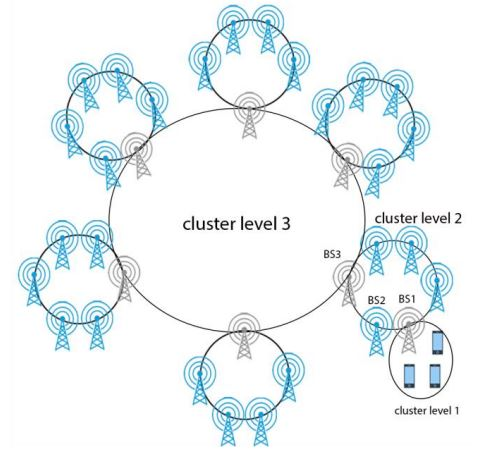
\includegraphics[width=10cm]{cluster-levels}}
	\caption{خوشه‌بندی سه‌لایه‌ای از ایستگاه‌های پایه}
	\label{fig:cluster-levels}
\end{figure}

\begin{figure}[ht]
	\centerline{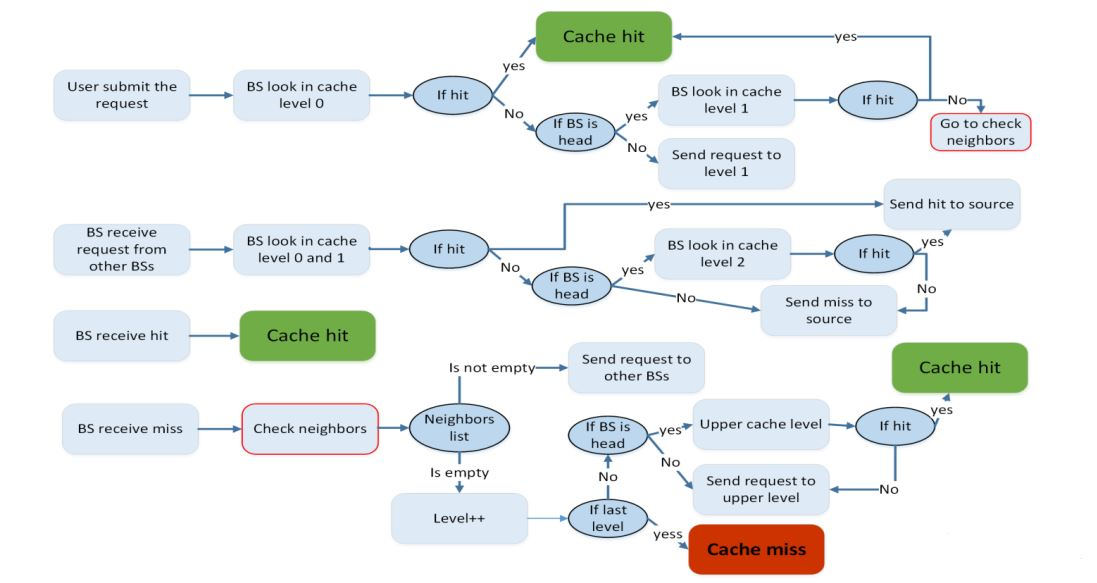
\includegraphics[width=14cm]{FDRL}}
	\caption{دیاگرام جریان داده برای پاسخ به درخواست‌های کاربران در مدل سلسله مراتبی و مشارکتی}
	\label{fig:fdrl}
\end{figure}

\begin{figure}[ht]
	\centerline{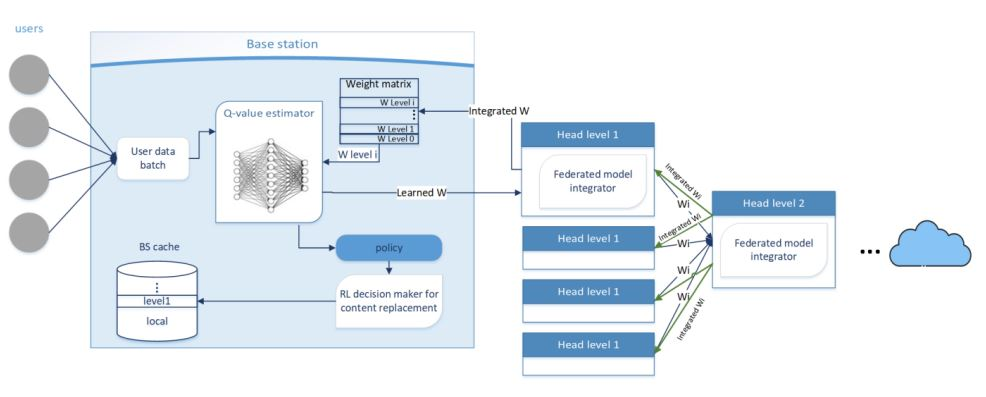
\includegraphics[width=14cm]{HFDRL}}
	\caption{مکانیزم تجمع مدل‌ها در معماری سلسله مراتبی فدراسیونی یادگیری تقویتی عمیق}
	\label{fig:hfdrl}
\end{figure}

